%SHAPE CLASSES \& FINANCIAL LITERACY - WORKSHEET 0 (IN-CLASS INSTRUCTION)
\documentclass[12pt, letterpaper, fleqn]{article}

% ----------------------------------------------------------
% PACKAGES
% ----------------------------------------------------------
\usepackage{graphicx}
\usepackage{xcolor}
\usepackage[most]{tcolorbox}
\usepackage{amsmath, amssymb}
\usepackage{fancyhdr}
\usepackage[utf8]{inputenc}
\usepackage[T1]{fontenc}
\usepackage{enumitem}
\usepackage{geometry}
\usepackage{tikz}
\usepackage{needspace}
\usepackage{multicol}

\usetikzlibrary{arrows.meta, calc, shapes.geometric}

% ----------------------------------------------------------
% PAGE SETUP
% ----------------------------------------------------------
\usepackage{times}
\geometry{letterpaper, top=1.25in, bottom=1.25in, marginpar=0.5in}

% ----------------------------------------------------------
% HEADER / FOOTER
% ----------------------------------------------------------
\newcommand{\logowidth}{3cm}
\setlength{\headheight}{20pt}
\setlength{\footskip}{40pt}

\pagestyle{fancy}
\fancyhf{}
\fancyhead[C]{\small\bfseries Shape Classes \& Financial Literacy}
\fancyfoot[L]{\raisebox{2pt}{
\includegraphics[width=\logowidth]{../kss.png}}}
\fancyfoot[C]{\thepage}
\fancyfoot[R]{3.25.0}

\renewcommand{\footrulewidth}{0.2pt}

% ----------------------------------------------------------
% THEME COLOR
% ----------------------------------------------------------
\definecolor{customteal}{HTML}{2fbdb9}

% ----------------------------------------------------------
% HELPER MACROS
% ----------------------------------------------------------
\newcommand{\blank}{\underline{\hspace{2.2cm}}}
\newcommand{\blanklong}{\underline{\hspace{6.5cm}}}
\newcommand{\blankshorter}{\underline{\hspace{1.5cm}}}

% ----------------------------------------------------------
% DOCUMENT
% ----------------------------------------------------------
\begin{document}

\textbf{Name:} \underline{\hspace{5cm}}
\hfill
\textbf{Date:} \underline{\hspace{3cm}}\\

\begin{tcolorbox}[colback=customteal!20]
    \large\textcolor{black}{\textbf{Quadrilaterals & Shape Partitioning}}
\end{tcolorbox}

\vspace{3mm}
\noindent
\textbf{Quadrilaterals} are shapes with 4 sides. 
\begin{itemize}
    \item **Rectangle:** 4 right angles.
    \item **Square:** 4 right angles and 4 equal sides.
\end{itemize}
We can partition (split) shapes into parts with **equal areas** (like halves, thirds, fourths).

\vspace{3mm}
\begin{tcolorbox}[colback=white, colframe=black!25, boxrule=0.6pt, arc=4mm]
\textbf{Financial Literacy: Coins & Bills}
\\
* Penny = 1\text{ cent}
* Nickel = 5\text{ cents}
* Dime = 10\text{ cents}
* Quarter = 25\text{ cents}
* Dollar Bill = 100\text{ cents}
\end{tcolorbox}

\newpage
\begin{tcolorbox}[colback=customteal!20]
    \large\textcolor{black}{\textbf{Guided Practice}}
\end{tcolorbox}

\vspace{5mm}
\begin{enumerate}[itemsep=3cm, leftmargin=0.6cm]
\item Partition the circle into 4 equal quarters.
\begin{center}
\begin{tikzpicture}[scale=0.8]
\draw[thick] (0,0) circle (1.2cm);
\end{tikzpicture}
\end{center}

\item Alice has 2 quarters, 1 dime, and 3 pennies. How much money does Alice have?
\\
Equation: \blank $+$ \blank $+$ \blank $=$ \blank cents
\end{enumerate}

\end{document}
